                 % Chapter Template

\chapter{Belief Management} % Main chapter title

\label{chapter:belief_management} % Change X to a consecutive number; for referencing this chapter elsewhere, use \ref{ChapterX}

\lhead{Chapter 3. \emph{Belief Management}} % Change X to a consecutive number; this is for the header on each page - perhaps a shortened title

In this chapter we show how our system is able to manage agents beliefs. Section~\ref{sec:belief_management-intro} provides an introduction to the subject, with a discussion on some relevant works. Section~\ref{sec:belief_management-overview} shows an overview of our approach, discussing its key aspects and modules. Sections~\ref{sec:belief_management-system_inputs}  shows the simplified mechanism that we use to detect objects and humans. In section~\ref{sec:belief_management-geometrical_reasoning} we explain the geometrical reasoning capacities of our system, introducing the main symbolic facts that are computed. Finally, in section~\ref{sec:belief_management-belief_management} we show how we build human belief models starting from these facts.

\section{Introduction}
\label{sec:belief_management-intro}
%Motivation

In HRI, it is important to represent humans not as simple obstacles, but as acting entities, with different beliefs on the state of the world and with the capacity to affect the environment. 

A simple example to prove this point is related to proxemics. Normally, when we approach an object, like a table, in an empty environment, we just choose the quickest path. If, intead, the environment is populated by other people, we will follow a set of social rules, like keeping a certain distance from them. If the robot does not follow these rules, it might freighten people, for example by approaching quickly from behind the person, or be considered as `rude'.


Theory of Mind~\citep{premack1978does} is a skill used to reason about humans' beliefs and thoughts, and how they affect actions. An ability linked to this concept is perspective taking, which is widely studied in developmental literature.  Flavell in \cite{flavell1977development} describes two levels of perspective taking: 
perceptual perspective taking, the capacity to understand that other people see the world differently \citep{Tversky1999}; and conceptual perspective taking, the capacity to attribute thoughts and feelings to other people \citep{Baron1985}. 

Through perceptual perspective taking we are able to compute information such as `I can see the glasses, but you can not', `you can reach the bottle, but I can not'. Conceptual perspective taking is equally important, and allows us, for example, to understand that a friend, when choosing the flavors for its ice cream, would choose its favourites, which might differs from ours.

An important study linked to conceptual perspective taking is the \textit{divergent belief task}.  Formulated in~\cite{wimmer1983}, this kind of task requires the ability to recognize that others can have beliefs about the world that differ from the observable reality.  A typical test used to study divergent belief is the Sally and Anne test (Figure~\ref{fig:belief_management-sally_anne}). In this test, Sally and Anne are two puppets. A short scene is shown to participants, where Sally takes a ball and hides it in her basket, before leaving the room. While she is away, Anne takes the ball from Sally's basket and puts it in her  box. After Sally returns, participants are asked a question: ``Where will Sally look for her object?''. Young children, or those affected by autism, might answer (wrongly) that Sally will look for her object in Anne's box, not taking into account that she does not know that it was moved.

 \begin{figure}[ht!]
	\centering
	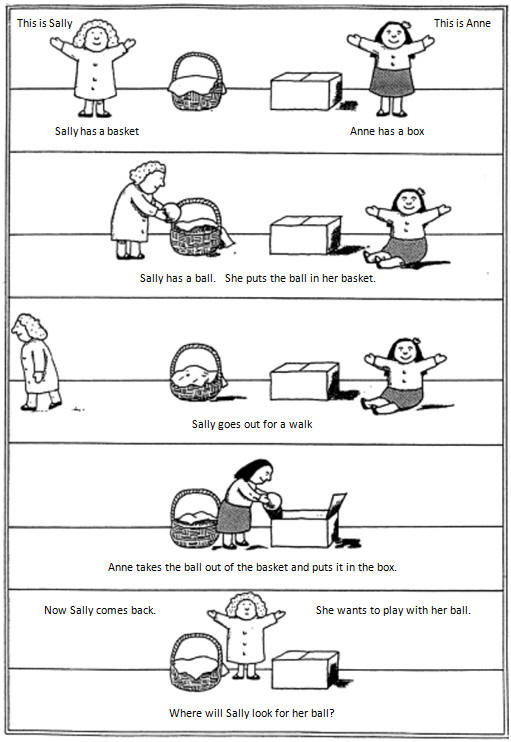
\includegraphics[scale=0.45]{img/observer/sally-anne.jpg}
	\caption{The Sally and Anne test. Original artwork by Axel Scheffler.}
	\label{fig:belief_management-sally_anne}
\end{figure}

Studies on individuals that do not possess the required mechanisms to perform perspective taking \citep{frick2014picturing} have shown that they encounter great difficulties in social relationships, confirming the importance of this ability.

These studies make us think that perspective taking could be very important in robotics. For example, let us imagine a scenario where Greg and a robot are performing some household repairs, which require the use of different tools. The robot might create a plan to achieve this goal where the human needs to use a screwdriver, which is actually behind a box, hidden from the sight of  Greg. Without perspective taking, the robot will procede in its task while Greg is desperately looking for the screwdriver. By using perspective taking, instead, the robot would infer that Greg does not know where the screwdriver is, and can not see it. In this situation, the robot might inform Greg of the location of the screwdriver, give it to him, or create a plan where Greg does not need to use it, thus being a more likable helper.

Previous works in robotics have actually demonstrated that enhancing the robot's perspective taking abilities improves its reasoning capabilities, leading to more appropriate and efficient task planning and interaction strategies \citep{Trafton2005,ros2010one,breazeal2006}. Let us review some implementations of perspective taking.

The HAMMER system, previously presented in chapter~\ref{chapter:introduction}, has been extended in~\cite{johnson2005perceptual} to introduce perceptual perspective taking, using the concept of forward and inverse visual models. Forward vision models analyze sensory data to produce information, like the geometrical coordinates of objects. Inverse visual models, instead, receive as input desired properties and states (for example, the presence of objects of a certain shape and color in a particular location), and try to produce an appropriate visual image that respects these inputs.

Perspective taking is performed by introducing two forward vision models. The first one produces the location and relationships between objects and end effectors (like grippers), while the second  computes the gaze direction of other agents. Using the results of these models as input of an inverse visual model, the system can reconstruct the scene as seen by another agent. The representation of knowledge by agents is not explicitly handled in the system. 

The architecture of~\cite{BreazealGB09}, also presented in chapter~\ref{chapter:introduction}, is another cognitive system which uses simulation mechanisms, but the work  includes both perceptual and conceptual perceptive taking. In this system the robot's schemas are used to build its mental model and execute its tasks, but also to build humans mental models and infer their actions and goals.

The robot is able to build a belief on the world state by analyzing perceptual data, producing symbolic information, such as the location or color of an object. This belief is constantly maintained, by adding new information and erasing those that are no longer valid.

To build a belief model of a human, the robot manipulates perceptual data, by filtering objects that can not be seen by the human (because they are occluded, for example), and transforming the data to simulate a first-person experience on the human. By using the same mechanisms to manage the belief for itself and for humans, the robot can infer divergent belief situations. This method has been tested on variants of the Sally and Anne test with good results.

The belief management algorithm of this systems does not take into account information that can not be directly perceived, but must be inferred. For example, in a domestic scenario, a human might not be aware that a mug containing liquid is hot and should not be touched. These aspects could be inferred by taking into account the results of actions, like pouring hot liquid in the mug.

Another system able to model agent beliefs is~\cite{scheutz2013computational}. This work is oriented toward problems where a distributed team of agents needs to communicate over a remote connection to solve a task. Each agent is assumed to be able to create its own mental model using its perception capacities, even though the precise rules for these mechanisms are not explained. When an agent receives information, he updates his mental belief using a set of rules, introducing the new data and checking for incongruencies with his previous information.  Using the same mechanism, each agent forms a belief model of other agents that have received the same information.

We created a rule-based approach for belief management, based on geometric reasoning and on inference, which we will introduce in the following sections. 

\section{Belief Management Overview}
\label{sec:belief_management-overview}

\subsection{Process overview}

Managing beliefs means being able to build and maintain a model of the belief of each agent. Our system is able to accomplish this task with different steps.

Of course, to reason on the current situation the system needs to be able to detect humans and objects in the environment. In some case, to be generic, we will call an agent or an object an \textit{entity}. Section~\ref{belief_management:entity_detection} will show how detect and track entities.

We can assign \textit{attributes} to entities, parts of entities (e.g. the arm of a human), and areas to represent different information, like properties, the state of entities or relationships between entities. Examples of attributes are:
an agent can be in a specific area; a box can be opened and can contain objects; a bottle can contain liquids; a mug can be hot; a room can be a silent area, where the robot should avoid making any noise.
We divide attributes in two classes, which influence the capacity of agents to perceive them: 
\begin{itemize}
\item Fully observable. These attributes can be observed by any present agent looking at the linked entity or area (e.g. the box is open, Greg is in the kitchen).
\item Partially observable. These attributes can be observed by present agents only in specific situations, represented as rules linked to the object and the attributes, e.g. an agent can see that a box contains items only when it is open, an agent can detect that the mug is hot only when he touches it. 
\end{itemize}

The locations of entities are integrated with other data produced by sensors through geometrical reasoning in order to produce symbolic informations, such as spatial relationships between objects and humans. We represent these information as facts. A fact is a tuple $subject\> predicate\> value$, which we use to represent symbolic knowledge. An example of fact is $CUP\> isOn\> TABLE$, which defines the location of an object. The instance of an attribute is represented as a fact, and so, each fact will correspond to exactly one attribute. More details about this aspect will be shown in section~\ref{sec:belief_management:geometrica_reasoning}.

We call \textit{world state} the collection of all facts describing the current situation. A \textit{belief model} is a collection of facts representing the knowledge of an agent on the world state. Each agent can have a different belief model, since the environment can change without an agent being able to perceive it. To represent the lack of knowledge of an agent, the value of a property can be \textit{unknown}. For example, the robot could take a tool from the table, while Greg is in another room, and place it in a box. Greg has not seen this event, and so his belief model will contain the (wrong) information that the tool is still on the table.  Section~\ref{sec:belief_management-belief_management} will show in, details, our approach to update the belief model of an agent.

In general, beliefs models are updated when the system infers that an \textit{action} has been executed, bringing a change to the environment.  We define an action as a tuple $(name, preconditions, target, postconditions)$. The $name$ of an action is a unique string that identifies it. The $preconditions$ are a set of facts that must be true in order to realize the action. In our system, an action is executed on a $target$, which can be a physical object, like a cup, but also an area of the environment, like a room. The $postconditions$ are the set of facts, and their values, affected by the action's execution.  


Since we are interested on reasoning and not perceptual aspects, we use inference, as explained in section \ref{sec:belief_management-intention_recognition}, in order to understand when a human has performed an action. Through the predefined $postconditions$ of actions we can also infer changes in the state of objects, e.g. the human opens a box, so the box is now open. 


\subsection{Architecture}
These aspects are represented in the Situation Assessment layer, and in particular in the following modules, shown in figure~\ref{fig:belief_management-belief_management_overview}.

\begin{itemize}
\item Sensor Data. Data produced by different possible sensors (e.g. lasers, camera, etc.).
\item Entity Detection. Different components detect and track humans and objects in the environment.
\item Geometrical Reasoning. Symbolic facts are produced starting from perceptual data.
\item Belief Management. The system maintains a mental model of each agent.
\item Database. The Database stores symbolic facts produced by the system.
\item Intention and Action Recognition. The system infers the current intentions of a human, and which actions are executed, by integrating  geometrical reasoning, the human's belief model, planning, and bayesian inference.
\end{itemize}

 \begin{figure}[ht!]
	\centering
	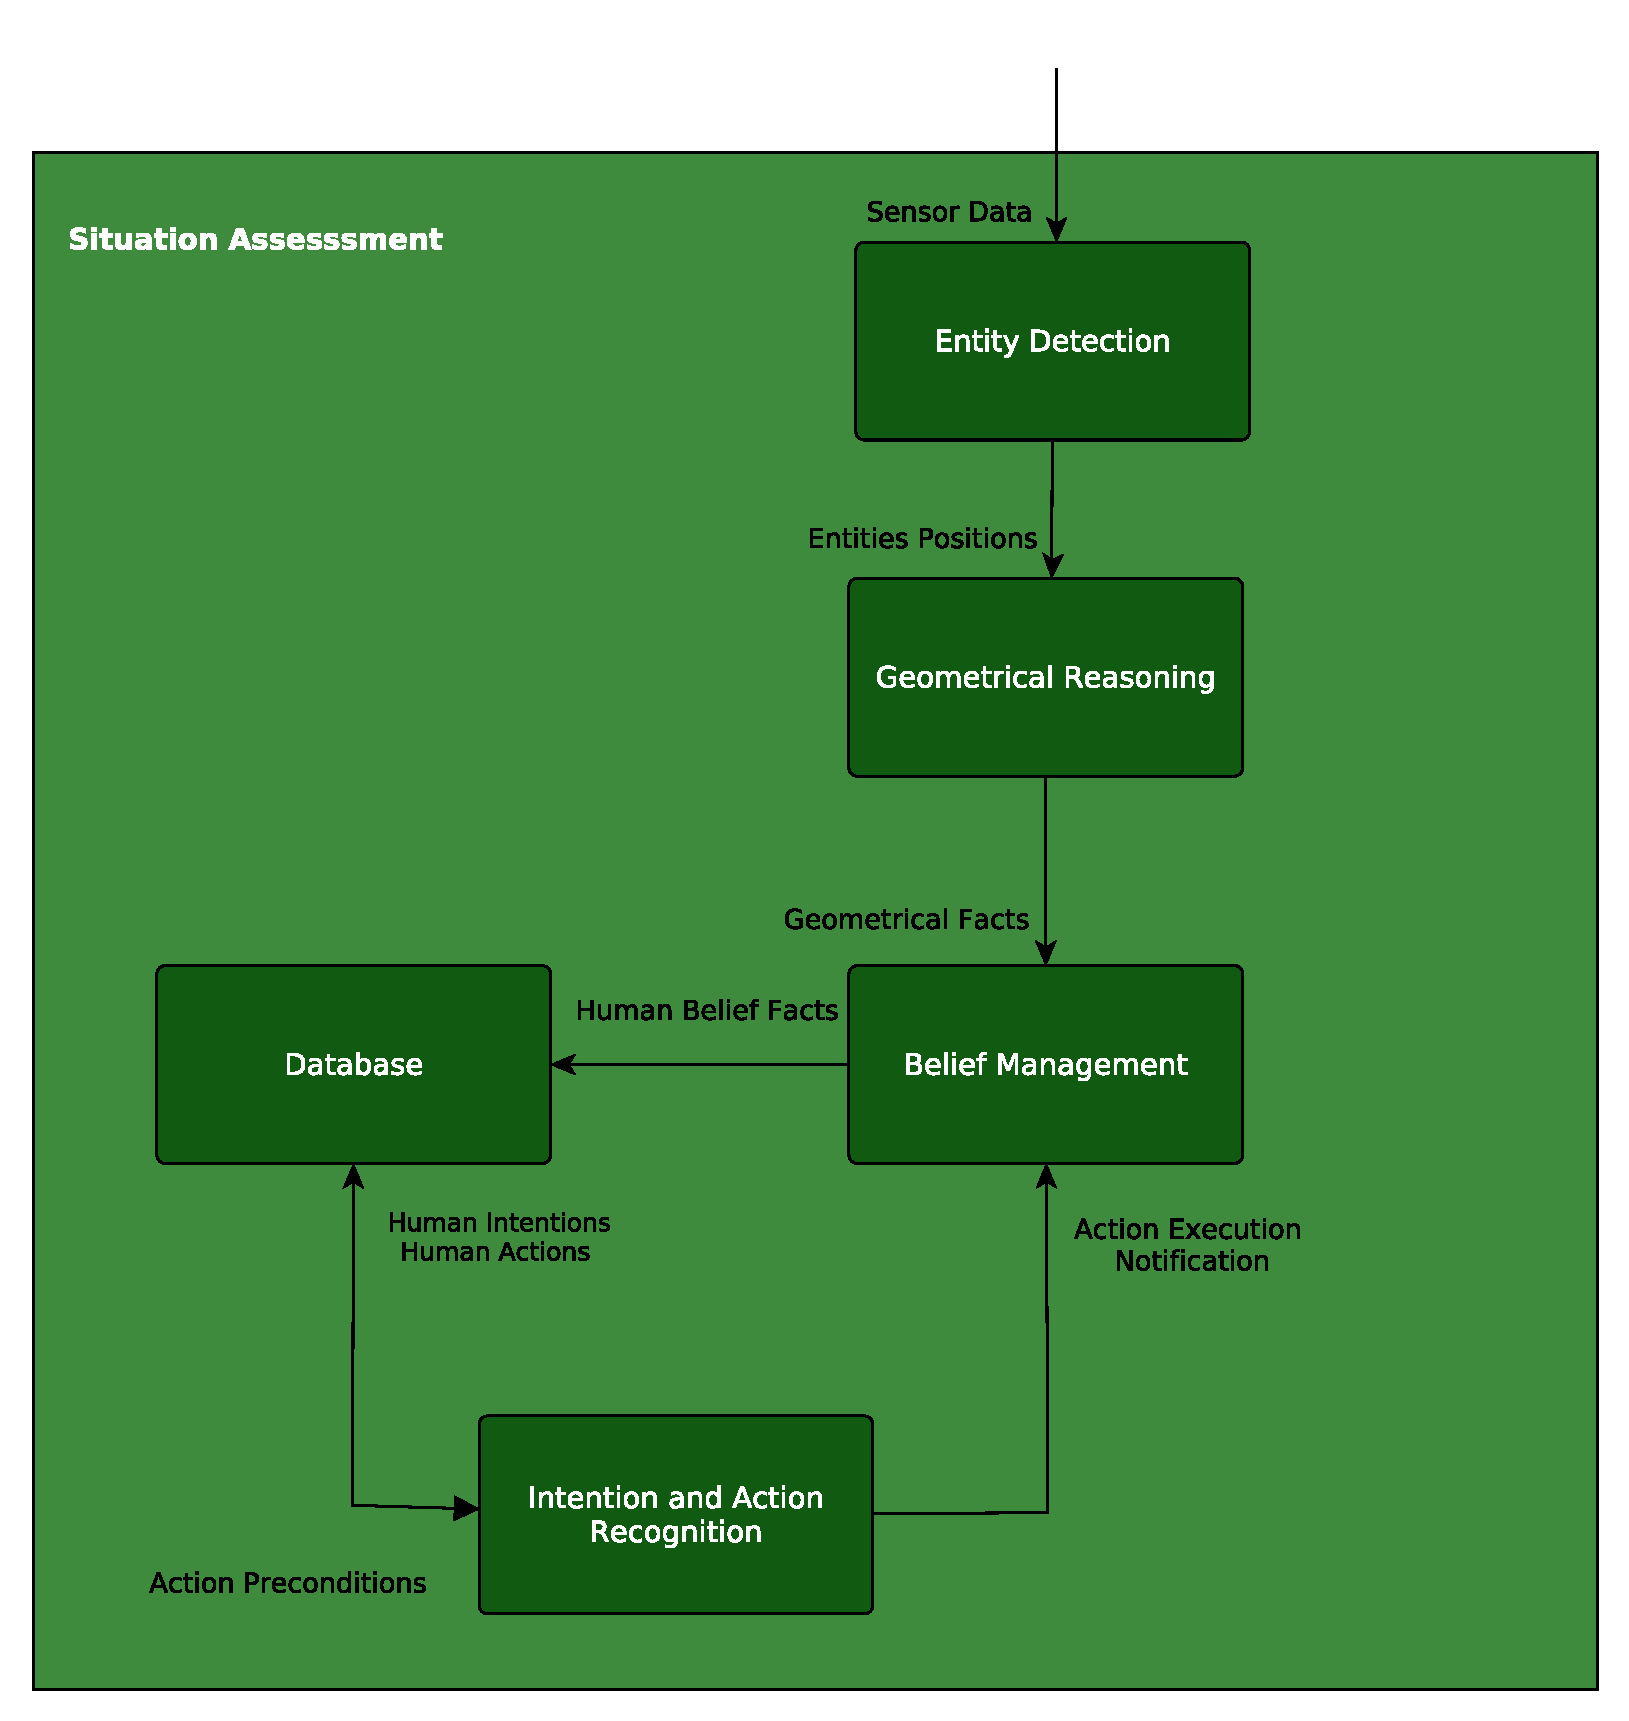
\includegraphics[scale=0.45]{img/observer/situation_assessment_overview.pdf}
	\caption{Overview of the different modules composing the Situation Assessment layer}
	\label{fig:belief_management-belief_management_overview}
\end{figure}

Symbolic facts are constantly produced, starting from the sensor data and from the position of entities. The Belief Manager collects these information to maintain the belief model of each agent. The belief model of humans and of the robot is used by the Intention and Action Recognition module to infer the most likely human intentions, and which actions they perform. All these information are introduced in the Database, and can be read by other components. For example, the Goal Management layer can choose a goal based on human commands or an estimation of humans' intentions. In a similar way, the Task Execution layer will read the Database in order to obtain the state of the world, to check action preconditions.  

The geometrical reasoning and belief management capacities of this layer were presented in \cite{Milliez2014}, where they were used to pass the Sally and Anne test~\cite{Baron1985} on a robotic platform. 

Dialogue can be a very important source of information. Agents often communicate, while executing a task together, or even when working independently, to clarify ambiguities and obtain missing information. While we will not present a specific dialogue component in this work,  in \cite{Ferreira2015} our belief management component was integrated with a situated dialogue system in a simulator. This model was compared with a basic system (without belief awareness) in a study with 60 interactions, in a simulated environment. We successfully showed that the dialogue management system significantly improves its efficiency, reducing the number of dialogue turns in the interaction, and its accuracy, with a higher success rate when a divergent belief situation appears.

In the following sections we will show how our system is able to manage agents' belief models. Actions will be treated, at this point, as input received by the Belief Management module. The intention and action recognition capacities of our system will be explained in~\ref{chapter:intention_recognition}. 

\section{Entity Detection}
\label{sec:belief_management-entity_detection}
In our system, we chose to simplify perception issues, focusing on reasoning aspects. We associate a unique tag to every object that is interesting in a particular scenario. When the robot observes a tag using a camera, it detects the corresponding object using a tag-matching algorithm.
Regarding humans, we use a motion capture software to identify and track agents moving in the environment. Using different tags, we can track the head, shoulders, and right arm of a human. Our situation assessment component has also been tested using a laser and RGB based detector, detailed in~\cite{lindermulti}, in the SPENCER european project. We also experimented using a depth camera, mounted on the ceiling, and a color-recognition algorithm to identify humans. 

 \begin{figure}[ht!]
	\centering
	\includegraphics[scale=0.7, trim={0 3cm 0 0}]{img/observer/explore.pdf}
	\caption[The robot builds a representation of the environment]{The robot explores the environment, recognizing objects through tags, and building a representation of the environment.}
	\label{fig:belief_management-explore}
\end{figure}

\section{Geometrical Reasoning}
\label{sec:belief_management-geometrical_reasoning}

Using its perception abilities the robot can build a representation of the environment, starting with entities' positions. With geometrical reasoning we can compute spatial relationships between entities, e.g. the glasses are on the shelf, the human is moving toward the library, the glasses are reachable by the human, the bottle is visible for the human. These reasonings provide a base for the perspective taking abilities of the robot.  The geometrical reasoning capacities of our system were introduced in~\cite{Sisbot2011}. This work was updated to include the production of new symbolic facts. We will show a list of some of the most important facts that our system is able to produce through geometrical reasoning.

\begin{itemize}
\item \textit{isOn}. Used when an object is on top of another, for example $CUP\; isOn\; TABLE$.
\item \textit{isNextTo}. Used when two objects are on the same surface and close to each other, for example $CUP\; isNextTo\; BOX$.
\item \textit{isReachable}. Used when an object is reachable by an agent, computed through inverse kinematics. An example of such predicate is $CUP\; isReachableBy\; ROBOT$
\item \textit{isVisible}. Used when an entity is visible by an agent. This is calculated by computing the field of view of an agent, and checking if there is a sufficient portion of the object not hidden by occlusions in this field. An example of this predicate is $CUP\; isVisibleBy\; ROBOT$.
\item \textit{isMoving}. Used when an agent is currently moving. This is computed by checking if the agent's displacements in a pre-determined time unit is bigger than a pre-determined threshold. We use an hysteresis filter to avoid continuous oscillation in the value of the fact. An example of $isMoving$ is $ROBOT\; isMoving\; TRUE$.
\item \textit{isMovingToward}. Used to indicate that an agent is moving toward a particular entity. This is computed by checking if the distance between the agent and the entity is decreasing. An example of this predicate is $ROBOT\; isMovingToward\; GREG$.
\item \textit{isOrientedToward}. Used to indicate that an agent is oriented toward a particular entity, for example $ROBOT\; isOrientedToward\; GREG$.
\item \textit{pose}. Used to indicate that an agent is in a particular pose, for example $GREG\; pose\; HANDOVER$.
\item \textit{isAt}. Used to indicate that an agent is in a particular location, for example $GREG\; isAt\; LIVING\_ROOM$.
\end{itemize}


\section{Belief Management}
\label{sec:belief_management-belief_management}
We have created a rule based framework in order to build the beliefs of each agent and update them when needed. Human belief models are updated using the perspective taking skills of the robot. When the robot detects the execution of an action in the world, with the mechanisms shown in chapter~\ref{chapter:intention_recognition},
it updates the belief model for itself and for every human that can perceive the action, adding its $postconditions$ to their models. When an action is not perceived by a human (e.g. the user was in another room), his belief model will not be updated, as he is not aware of the changes that occurred.

However, when he comes back and looks at the environment, we assign him a new belief state following a set of rules, which we will now explain. We call $p$ a fact, $H$ the agent, $HB$ his belief model, and $RB$ the robot's belief model. We also create the following predicates: $obs(p)$ means that $p$ is observable for $H$, $valid(p,x)$ means that $p$ does not contradict the current perception data of agent $x$, $value(p,m)$ is the value $p$ in belief model $m$, and $vis(p,x)$ means that agent $x$ has visibility on the linked entities of $p$ (e.g. if $p$ is $MUG\; isOn \; TABLE$ the linked entities are $MUG$ and $TABLE$) . The rules for the $valid$ predicate will be different in each attribute. For example the fact \textit{MUG isOn TABLE} will not be valid for agent Max if he can see that there is no mug on the table. For each fact $p\in HB \cup RB$:
\begin{itemize}
\item if $p \in RB, \quad p\not\in HB,\quad obs(p),\quad vis(p,H) \rightarrow value(p,HB)=value(p,RB)$.
\item if $p \not \in RB,\quad p\in HB,\quad obs(p),\quad vis(p,H) \rightarrow remove\quad $p$ \quad from \quad HB$.
\item if $p\in RB,\quad p\in HB$ then:
	\begin{itemize}
      \item if $value(p,HB)\neq value(p,RB),\\ \quad obs(p),\quad vis(p,H) \rightarrow \\ value(p,HB)=value(p,RB)$.
      \item if $value(p,HB)\neq value(p,RB),\\ \quad !obs(p),\quad !valid(p,H) \rightarrow \\ value(p,HB)=\textit{unknown}$.
	\end{itemize}
\end{itemize}
The idea of this set of rules is updating an agent's mental belief model for a fact only if it is observable, or if it is not observable and perception data contradicts the current value of the fact (e.g. the mug was moved from the table to the kitchen while the agent was in another room. While the agent can not see where is the mug, he can see it is no longer on the table).


%TODO: Image of perspective taking

